\section{A bit more commands}
% This is unique for class presentation.

\begin{frame}{tikz package}{http://www.texample.net/tikz/examples/tag/graphs/}
\begin{minipage}[b]{0.4\textwidth}
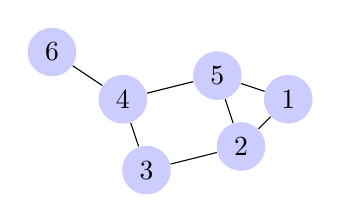
\begin{tikzpicture}
  [scale=.3,auto=left,every node/.style={circle,fill=blue!20}]
  \node (n6) at (1,10) {6};
  \node (n4) at (4,8)  {4};
  \node (n5) at (8,9)  {5};
  \node (n1) at (11,8) {1};
  \node (n2) at (9,6)  {2};
  \node (n3) at (5,5)  {3};

  \foreach \from/\to in {n6/n4,n4/n5,n5/n1,n1/n2,n2/n5,n2/n3,n3/n4}
    \draw (\from) -- (\to);

	\end{tikzpicture}
	\end{minipage}
	\begin{minipage}[b]{0.4\textwidth}
	    \begin{block}{}
	    	Very useful package for graphics and such. \\
			But this is not something I will go into detail in.
		\end{block}
	\end{minipage}
\end{frame}

\begin{frame}{More trees with qtree}{http://www.ling.upenn.edu/advice/latex/qtree/qtreenotes.pdf}
	\begin{minipage}[b]{0.4\textwidth}
	\footnotesize
		\Tree[.IP [.NP [.Det \textit{the} ]
               [.N\1 [.N \textit{package} ]]]
          [.I\1 [.I \textsc{3sg.Pres} ]
                [.VP [.V\1 [.V \textit{is} ]
                           [.AP [.Deg \textit{really} ]
                                \qroof{\textit{to use}}.CP ]]]]]
    \normalsize
	\end{minipage}
	\begin{minipage}[b]{0.4\textwidth}
	    \begin{block}{}
	    	Very useful package for graphics and such. \\
			But this is not something I will go into detail in.
		\end{block}
	\end{minipage}
\end{frame}

\begin{frame}[fragile]{Image placement - Place images anywhere?}{http://staff.www.ltu.se/~johanc/teaching.htm}
	\begin{minipage}[b]{0.4\textwidth}
	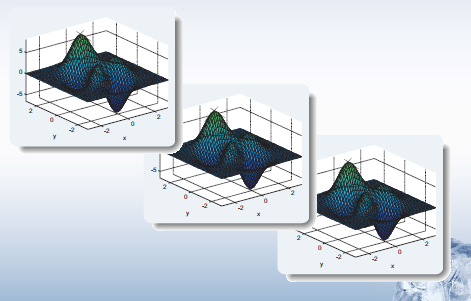
\includegraphics[width=\textwidth]{img/4-imagefloat.png}
	\end{minipage}
	\begin{minipage}[c]{\textwidth}
	    \begin{block}{}
	    	\begin{lstlisting}
				\putimageblock{.55}{.95}{.25}{peaks.pdf}
				\putimageblock{.35}{.80}{.25}{peaks.pdf}
				\putimageblock{.15}{.65}{.25}{peaks.pdf}
			\end{lstlisting}
		\end{block}
	\end{minipage}
		
\end{frame}